% ==============================================================================================
% 2010-11-05 Preisig, H A       ; NTNU
% 2011-12-15  ditto             ; adapted for PSE 11
%                               ; put all the heading info into the style file
% 2012-01-04  ditto             ; Reference section title fixed -- integrated into style file
%                               ; changed sequence: first bibliography then pse style
%                               ;  pse style redefines reference listing superseding natlib def
%                               ;  and simplified by moving reference style loading into pse.sty
% 2014-09-04  ditto             ; reverted to standard LaTeX fonts
%                               ; issues - measures do not correspond with manual. 
%                               ; There is a cm missing 13.5 textwidth gives 12.5 texwidth ???
% 2015-10-14 Zinser, A          ; adapted to ESCAPE 26
% ==============================================================================================

\documentclass[fleqn,twoside,10pt]{article}

%% bibliography must be before escape styles
\usepackage{natbib}

%% Escape/PSE styles
\usepackage{left_eq}   % To get the equation left aligned, this is ugly but required :-)
\usepackage{pse2018}  % Stylefile from Escape


%%% >>>>>>>>>>>>>>> use your own GRAPHICS configuration <<<<<<<<<<<<<<<<<<<<<<<
\usepackage{pstricks, pst-plot}	% pstricks
\usepackage{graphicx} % enables import of various formats
\usepackage{wrapfig}  % enables floating wrapped figures
\usepackage[figuresright]{rotating}
\usepackage{amsmath}
\usepackage[font=sf, labelfont={sf,bf}, margin=0cm]{caption}
\usepackage[inline]{enumitem}
\usepackage{epstopdf}   
%\usepackage[margin=1in]{geometry}
\usepackage{lineno}
\usepackage{placeins}
\usepackage{subcaption}
%\usepackage[usenames,dvipsnames]{color}
%\usepackage[usenames,dvipsnames,svgnames,table]{xcolor}
\usepackage{algorithm}
\usepackage{algpseudocode}
\usepackage{textcomp}
\usepackage{graphicx}
\usepackage{tabulary}
\usepackage{wrapfig}
\usepackage{lipsum}
\usepackage{lineno}
%% math packages
\usepackage{amsmath}
\usepackage{amssymb}
\setlength{\mathindent}{0.1cm}


%% >>>>>>>>>>>>>>>> user definitions BIBLIOGRAPHY & DEFS <<<<<<<<<<<<<<<<<<<<<<<<


%% personal styles and definitions
%\usepackage{mystyle}
%\def\mydefs{defs}
\usepackage[english]{babel}
\usepackage{blindtext}


% ================================================================================
\title{Parallel, multi-scale, mechanistic model for high shear granulation using
coupled DEM-PBM models on high performance computing systems.}
%
 \author[a]{Chaitanya Sampat}
 \author[a]{Yukteshwar Baranwal}
 \author[b]{Ioannis Paraskevakos}
 \author[b]{Shantenu Jha}
 \author[a]{Marianthi Ierapetritou}
 \author[a,*]{Rohit Ramachandran}
 \affil[a]{Department of Chemical and Biochemical Engineering, Rutgers University, Piscataway, NJ-08901, USA}
 \affil[b]{Electric and Computer Engineering, Rutgers University, Piscataway, NJ-08901, USA}
 \email{*rohitrr@soe.rutgers.edu}
 
 \HeaderTitle{Parallel, multi-scale, mechanistic model for high shear granulation using
coupled DEM – PBM models on high performance computing systems.}
 \HeaderAuthor{C. Sampat et al.}

% ==================================== title ====================================

\begin{document}

\maketitle             % make title page with abstract and keywords
\thispagestyle{empty}  % first page has a different format

% ================================================================================

\begin{abstract}
A multiscale model combines the computational efficiency of a macro-scale model and the
accuracy of a micro-scale model. It is preferred over a fully micro-scale model for its speed advantages while maintaining the physics 
of the problem. A less accurate way to perform such a simulation is to use data 
from a precomputed microscale model in a macroscale 
model. With the current cyberinfrastructure resources available, using more computationally intensive and concurrent multiscale models 
are more feasible This study proposes to use Discrete Element Method (DEM), a 
microscale model, and a Population Balance Model (PBM), 
a macroscale model, in a concurrent manner to model the granulation process of a pharmaceutical product inside a high shear 
granulator. The granulation between the components of a pharmaceutical blend is governed by the collision in between the particles. 
This leads to increase in their size, due to physical bonds in between them. The DEM provides the collision data while the PBM helps 
in predicting the macroscale phenomena like aggregation and breakage. This work attempts to couple these two models using a controller 
program, which triggers the DEM first, to give initial seed data to run the PBM. Then, the controller uses the data generated from the 
PBM continuously to determine the change in the physical properties and trigger the DEM from its last known state. The controller does 
the same with the DEM data to trigger the PBM. This occurs iteratively until a steady state is reached. A workflow diagram of the 
procedure followed is provided in Figure 1. The execution of each of the components is governed by a multilevel job scheduler which 
allocates resources rather than waiting for each simulation to run on a
normal job scheduler on a cluster. The DEM is parallelized using Message Parsing Interface (MPI) while the PBM is parallelized using a 
faster hybrid approach which is a combination of both MPI and Open Multi-Processing (OMP). Since the DEM is computationally heavy, an 
algorithm is developed to utilize the idle cores during the PBM execution to run multiple instances of the PBM such that parameter 
estimation of the kernels of the PBM occurs on the fly as well. This method of using shorter bursts of each simulation led to faster 
simulation times as well as a more accurate model of the high shear granulator. The Quality by Design (QbD) approach is addressed 
using such a modeling framework and it also helps us understand the
granulation process in a quantitative as well as in a mechanistic manner.
\end{abstract}
\Keywords{Multi-scale Model, Population Balance Model, Discrete Element Method, High-performance computing, MPI}

% ==================================== body  =====================================
%\linenumbers
\section{Introduction}
Particulate materials are products or intermediates of around $60\%$ of the 
chemical industry~\citep{ingram2005}.
The modeling of these particulate processes pose a challenge when compared to 
modeling if uniform liquid
systems. These solid systems usually comprise of solids which co-exist with various sizes and shape configuration,
which have a large effect on the final composition and the performance of the product. This variation in the 
configuration of the product is unacceptable by the pharmaceutical industry. It 
could lead to differences in the 
dissolution rates and bioavailability of the product thus, affecting the quality of the product. The unit process 
that helps control the size of a granule of the powder in the pharmaceutical product is granulation. During this 
unit operation, fine powders are converted to the  larger particles by the process of aggregation. This occurs
due to addition of a liquid binder, making the particles agglomerate into larger granules. This process is also 
referred to as wet granulation as a liquid binder is added. Due to high restrictions set by the Food and Drug 
Administration (FDA) these products undergo various batch rejections or have 
high recycle ratios~\citep{sen2014}. 
One of the major aims of the industry currently is to reduce this waste, thus creating a need for better 
modeling of this process.

The most popular way to model the granulation process is to use a population balance model (PBM). This model 
tracks the number of particles with certain set of characteristics such as 
size, porosity and liquid content. 
It also takes into account the changes that may occur in these properties due to growth, breakage, consolidation, 
and other phenomena. This model is discussed in more detail in 
section~\ref{sec_mthds_PBM}. PBM fails to account 
for the particle level data, thus being inaccurate at times. This particle level data needed to improve the PBM 
can be obtained from discrete element methods (DEM). DEM help obtain the velocity of each particle and the 
number of times it collides with other particles by solving the Newton's laws of motion. This information 
is vital to the PBM as it helps develop a more accurate model with a higher physical significance. As these 
methods are complementary to each other, they are usually coupled while 
building a model for the granulation 
process. These processes can be coupled serially like in \textbf{(cite current paper here)} or in parallel as 
discussed in this work. DEM is always executed at initiation and the particle level data is then transferred to 
the PBM. The DEM simulation is computationally very high as it needs to solve large amounts of simultaneous 
equations at every time step. The parallel execution of this type of coupling requires various instances 
of simulation of each of these models to be initiated, requiring high computational power. The most efficient way 
to make these simulations run faster is to take advantage of large number of CPU cores present on modern day 
high-performance computing systems (HPCs / supercomputers).

This work focuses on the building of physically accurate model for a high shear 
granulator. Section \ref{methods} 
discusses the model equation used and the method of parallelization implemented on the PBM and DEM to enable them to 
run on various cores of HPCs. The resulting particle properties from the coupling and the speed improvements 
achieved when the number of cores used for the simulation are changed, is discussed in section \ref{results}.

%\begin{itemize}
%\item Talk about pharmaceutical processes
%\item Talk about DEM and PBM
%\item Coupling and its importance
%\item Advantages of using HPC
%\end{itemize}

\section{Methods}
\label{methods}
Figure \ref{fig:mthds_flow_dia} represents the workflow followed for the two-way coupled model that was used to model 
the high shear granulator. A two-dimensional PBM was developed for the solids present while a lumped model was 
used for the liquid and gas content. The PBM tracked particle flow, aggregation, breakage, 
consolidation and liquid addition. This PBM used the particle velocities and collision data from the DEM simulations 
making it mechanistic in nature. The DEM simulation was used to obtain the 
particle residence time, velocities, inter-
particle as well as particle-geometry collisions. These simulations were monitored using python scripts to switch 
in between the two simulations. The details of each of these components are discussed in this section. 

\begin{wrapfigure}[30]{R}{0.45\textwidth}
\centering
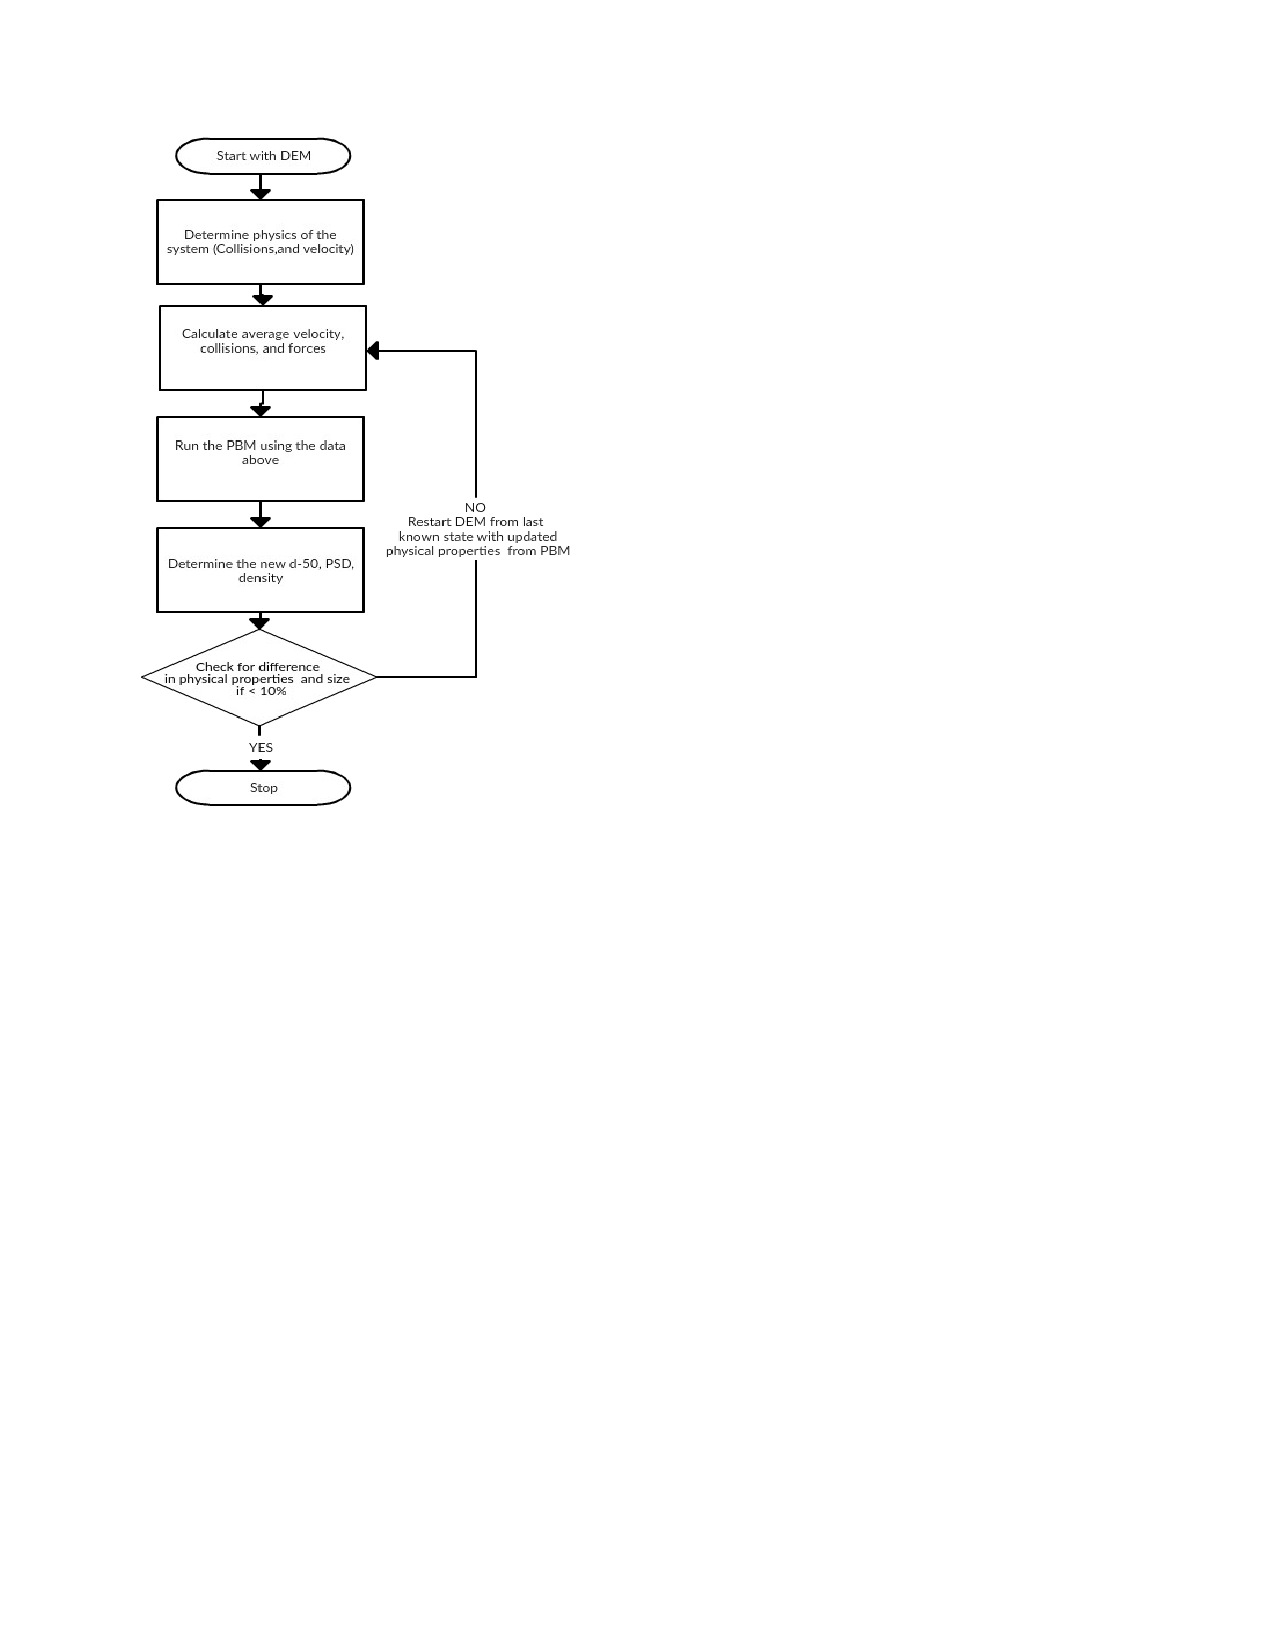
\includegraphics[scale=1]{flo_dia.pdf}
\caption{Schematic of the bi-directional approach used to model the high shear granulator.}
\label{fig:mthds_flow_dia}
\end{wrapfigure}
\lipsum[0]
\subsection{Population Balance Model (PBM)}
\label{sec_mthds_PBM}
A detailed, mechanistic two dimensional PBM was developed in \textit{C++}, which tracked the particles as they 
undergo the aggregation, breakage, consolidation and liquid addition. The governing population balance model 
is shown in Equation \ref{eqn:PBM_governing}.
\begin{flalign}
\label{eqn:PBM_governing} 
&\frac{d}{dt}F(s_1,s_2,x)=\Re_{agg}(s_1,s_2,x) \\ \notag
&+\Re_{br}(s_1,s_2,x)+\dot{F}_{in}(s_1,s_2,x)\\ \notag
&-\dot{F}_{out}(s_1,s_2,x)
\end{flalign}

where, $F(s_1,s_2,x)$ is the number of particles with an active pharmaceutical ingredients (API) 
volume of $s_1$ and an excipient volume of $s_2$ in the spatial compartment $x$. The rate of 
change of number of particles with time in different size classes depend on the rate of aggregation $\Re_{agg}
(s_1,s_2,x)$ and the rate of breakage $\Re_{break}(s_1,s_2,x)$. Also, the rate of particles coming 
into, $\dot{F}_{in}(s_1,s_2,x)$ and going out, $\dot{F}_{out}(s_1,s_2,x)$ of the spatial compartment 
due to particle transfer affect the number of particles in different size classes. 

The aggregation and breakage kernel as defined in Equations \ref{eqn:PBM_agg_cons} and \ref{eqn:PBM_break_cons} 
respectively These mechanistic kernels used the DEM inter-collision data as 
well as the impacts with the geometry 
to determine the collision and impact rate. The velocity of these particles were used to create a velocity 
distribution which decided whether the particle agglomerated with other particles or had to undergo breakage due to 
the impact on the geometry. The further details about the aggregation and breakage kernels can be found in 
\cite{barrasso2015cerd}. Details about the lumped model for the gas and liquid present in the system 
can be found in \textbf{(Cite current paper)}.


\begin{align}
\Re_{agg}(s_1,s_2,x)&= \frac{1}{2}\int _0^{s_1} \int_0^{s_2} 
\beta(s_1',s_2',s_1-s_1',s_2-s_2',x)F(s_1',s_2',x)F(s_1-s_1',s_2-s_2',x)ds_1'ds_2'\notag\\ 
&- F(s_1,s_2,x)\int _0^{s_{max_1}-s_1} \int_0^{s_{max_2}-s_2} 
\beta(s_1,s_2,s_1',s_2',x)F(s_1',s_2',x)ds_1'ds_2'
\label{eqn:PBM_agg_cons}
\end{align}
where, the aggregation kernel, $\beta(s_1,s_2, s_1',s_2',x)$ is expressed as a function of collision 
rate coefficient ($C$) and probability that collision results in agglomeration($\psi$)

\begin{align}
\Re_{br}(s_1,s_2,x) = \int_0^{s_{max_1}} \int_0^{s_{max_2}} 
K_{br}(s_1',s_2',x)F(s_1',s_2',x)ds_1'ds_2' - K_{br}(s_1,s_2,x)F(s_1,s_2,x)
\label{eqn:PBM_break_cons}
\end{align}
%%	     \textcolor{red}{citation?}	    
where, the breakage kernel $K_{break}(s_1,s_2,x)$. 

The number of solid bins selected for this simulation were 16 for each type of 
solid. The granulator was 
divided in 16 axial compartments to help with the parallelization of the \textit{C++} code. Since each 
compartment needed to perform identical calculations which were independent each other, they could 
be sent different CPU cores without any decrease in the speed as there will be minimum communications 
between these processes for a given time step. Thus, each of compartment was sent to a single process 
(core) using message parsing interface (MPI). The PBM code was made to dump the d50 and number of 
particles at an interval of $0.2s$ such that the controller could monitor the 
execution. 

%
%\begin{align}
%\dot{g}_{cons}(s_1,s_2,x)=&c (\nu_{impeller})^{\omega}V(s_1,s_2,x)\frac{(1-\epsilon_{min})}{s} 
%\notag \\ 
%& \left[g(s_1,s_2,x)+l(s_1,s_2,x) -(s_1+s_2)\frac{\epsilon_{min}}{1-\epsilon_{min}}\right]
%\end{align}        
%
% where, $c$ and $\omega$ are the consolidation constants; $v_{impeller}$ is the impeller 
%rotational speed; $V(s_1,s_2,x)$ is the volume of particle, $\epsilon_{min}$ is the minimum porosity; 
%$g(s_1,s_2,x)$ and $l(s_1,s_2,x)$ are respectively the gas and liquid volumes of the particle.


%\begin{align}
%K_{break}(s_1,s_2,x) = C_{impact}\int_{U_{break}}^{\infty}p(U)dU    
%\end{align}



\subsection{Discrete Element Model (DEM) setup}
The DEM simulation was performed on an open-source DEM software known as 
LIGGGHTS~\citep{kloss2012}.
The DEM simulation has to be initiated using a input file which was generated using a python script 
which was developed. The python script also helped generate the multiple restart files which would 
be required to restart the DEM simulation during the parallel multi-scale simulation. LIGGGHTS 
natively supports parallelization using MPI, which helps divide the geometry into various smaller 
simulation boxes thus, making them run faster compared to a serial code. \\
The particles used in the DEM simulation were of diameter $2mm$ and were considered to be 
granular in nature. A non-cohesive elastic contact model was used to model the collisions between 
the particles. The particles were introduced at the entry of the geometry with a constant mass 
flow rate of 15 kg/hr. The impeller of the granulator was set to rotate at 2000 rotations per 
minute. This was kept so high since this would lead higher number of particles colliding with 
the walls of granulator leading to breakage of the particles. Physical 
properties of the particles 
required for the simulation were taken from \textbf{(cite current paper here)}. The collision and 
velocity data of the particles from the DEM simulation was printed at pre-decided intervals such 
that it could be monitored.

%\subsection{PBM parallelization technique}
\subsection{Controller development}
The controller scripts to monitor the DEM and PBM simulations were written in python. Each of these 
scripts was executed along with its respective simulation. The DEM controller script monitored the 
collision and velocity data being dumped by the DEM simulation. The data was first stored and the 
average of the velocities for each type of particles and the total number of collisions and impacts 
were determined. If there was a change in either of these properties of more 
than 15\%, an exit 
status was sent which led to killing the execution of the DEM and indicated to start the PBM 
simulation. The DEM controller script also printed out various data files required for the the PBM 
execution as well as for the restart of the DEM simulation if needed. In the case, the properties did  
not showing a variation of more than 15\% over the span of $5s$ of DEM simulation time, it was 
considered to be in steady state and that all the simulation were halted.\\
The PBM controller read the d50 and number of particle files which were printed by the PBM after a 
constant time interval. The change in each of these properties in each compartment was monitored 
and an exit signal was sent if they varied by more than 15\%. The halting of the PBM was accompanied 
by the printing of files required to restart DEM with new diameters and data for restarting the PBM 
if needed after the DEM simulation.  

\subsection{RADICAL-Pilot (RP)}
Running several simulations that are dependent on High Performance Computing (HPC) resources can 
be extremely time consuming, since each simulation must be submitted in the resource independently.
This can lead to varying queuing times. RADICAL-Pilot (RP) is a framework that implements the Pilot 
abstraction~\cite{pstar12}, where a container job is submitted to the HPC 
resource, the Pilot,
and once the necessary computing resources are being acquired they can be used to execute multiple
simulations by reusing the same resources. By utilizing RADICAL-Pilot, we implemented an execution
framework that allows to utilize the components described above. In addition, RP provides the necessary
instructions to terminate or restart the execution of DEM or PBM simulations based on decisions
made from the various controlling components.

%A major challenge faced while running large number of simulations was the communication between 
%various componenets of the system. Since each of these simulations were run on a high-performance 
%computing (HPC) resource, each component has to be submitted as an individual job and sually leading 
%to a mismatch in the sequence of execution of the jobs. This leads to each job halting before 
%completion until other componenets finish execution. This communication and job scheduling can be 
%overcome using pilot job abstraction. RP is a pilot job abstraction container developed at Rutgers' 
%electrical and computer engineering department, which supports scalable and efficient launching of 
%heterogeneous tasks across different platforms. RP helped create a link between each of these 
%components. The pilot also handled halting of the executions of the components when indicated by the 
%controller as well as the restart of the DEM and PBM whenever required. This also helped bypass the 
%waiting in multiple job-queues that would have been required to run multiple instances of these simulations.

\section{Results}
\label{results}
<<<<<<< HEAD
This coupled DEM-PBM simulation were tested on the Stampede2 supercomputer with the Knights Landing 
configuration. Each of the compute node of the cluster consists of Intel Xeon Phi 7250 
(\textquotedblleft Knights Landing\textquotedblright) which has 68 cores on a single socket 
clocked at 1.4 GHz, with 96 GB of DDR4 RAM. Each of the cores consists of 4 hardware threads. 
The simulations were run on various configuration of the cores used for each of the 
component of the system. The number of cores used for the DEM simulation varied from 16 to 256, 
while the PBM used cores from 1 to 16. The DEM and PBM controller scripts used 1 process each for 
their respective executions.\\
The coupled system took \textbf{X} DEM and \textbf{Y} PBM simulations to reach steady state. The 
total simulation time of DEM execution was \textbf{A} seconds and PBM was \textbf{B} seconds. 
%Discuss how many instances of the simulation of each occured 
=======
Discuss how many instances of the simulation of each occurred
>>>>>>> 59acc51d052c5dc3dfe767a32229d54514c9d0d1
\subsection{Scaling results}
Cores used for DEM and PBM and how scaling occured
\subsection{Improved results over one way coupling}
Better d50 plots particle count
\section{Conclusion}

% ================================ references ===================================
%% References 
%\section*{References} 
\bibliographystyle{elsart-harv}
\bibliography{pse2018_psl}
\end{document}
% ================================== end =========================================